% ------------------------------------------------------------------
%  Figura: Ingeniería Inversa FanLamp — 3 fases + tabla comandos (slide 21)
%  Compilar:  pdflatex 21_fanlamp.tex
% ------------------------------------------------------------------
\documentclass[tikz, border=0.2cm]{standalone}
\usepackage[utf8]{inputenc}
\usepackage[T1]{fontenc}
\usepackage{libertine}
\usepackage{xcolor}

\definecolor{primary}{HTML}{280091}
\definecolor{secondary}{HTML}{4C5CC5}
\definecolor{accent}{HTML}{3FCFD5}
\definecolor{exgreen}{HTML}{00B299}
\definecolor{darkgray}{RGB}{80,80,80}

\begin{document}
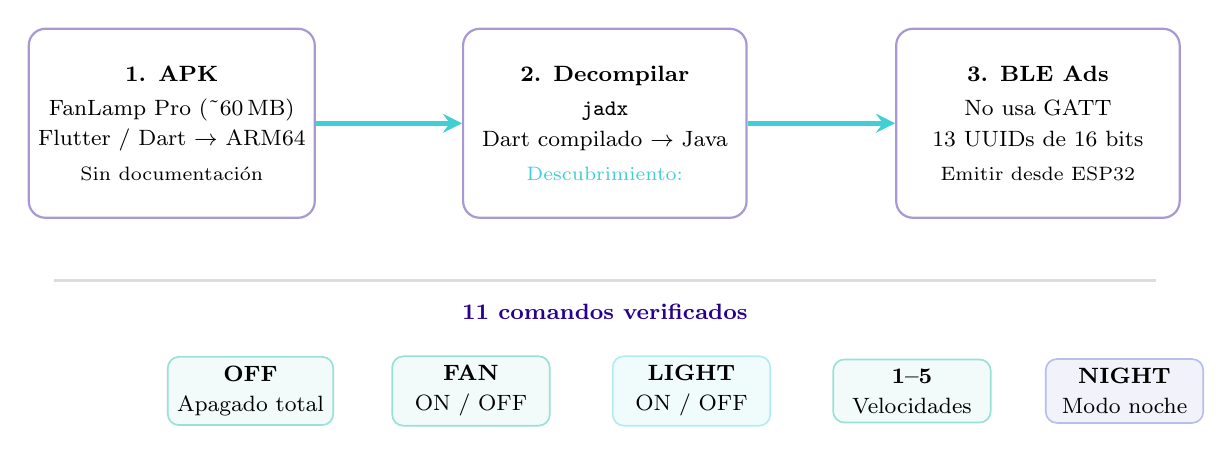
\begin{tikzpicture}[
    phase/.style={draw=primary!40, fill=white, rounded corners=6pt,
                  minimum width=3.6cm, minimum height=2.4cm, align=center,
                  font=\footnotesize, line width=0.8pt},
    arrow/.style={draw=accent, line width=2pt, ->, >=stealth},
    cmd/.style={draw=exgreen!40, fill=exgreen!5, rounded corners=4pt,
                minimum width=2cm, minimum height=0.8cm, align=center,
                font=\footnotesize, line width=0.6pt},
]

% Fase 1
\node[phase] (f1) at (0, 0) {
    \textbf{1. APK}\\[0.1cm]
    FanLamp Pro\ (\textasciitilde60\,MB)\\[0.05cm]
    Flutter / Dart $\to$ ARM64\\[0.1cm]
    {\scriptsize Sin documentación}
};

% Fase 2
\node[phase] (f2) at (5.5, 0) {
    \textbf{2. Decompilar}\\[0.1cm]
    \texttt{jadx}\\[0.05cm]
    Dart compilado $\to$ Java\\[0.1cm]
    {\scriptsize \textcolor{accent}{Descubrimiento:}}
};

% Fase 3
\node[phase] (f3) at (11, 0) {
    \textbf{3. BLE Ads}\\[0.1cm]
    No usa GATT\\[0.05cm]
    13 UUIDs de 16 bits\\[0.1cm]
    {\scriptsize Emitir desde ESP32}
};

% Flechas
\draw[arrow] (f1) -- (f2);
\draw[arrow] (f2) -- (f3);

% Resultado: tabla de comandos
\draw[darkgray!20, line width=1pt] (-1.5, -2) -- (12.5, -2);
\node[font=\footnotesize\bfseries\color{primary}] at (5.5, -2.4) {11 comandos verificados};

\node[cmd] at (1, -3.4) {\textbf{OFF}\\[0.05cm] Apagado total};
\node[cmd] at (3.8, -3.4) {\textbf{FAN}\\[0.05cm] ON / OFF};
\node[cmd, fill=accent!8, draw=accent!40] at (6.6, -3.4) {\textbf{LIGHT}\\[0.05cm] ON / OFF};
\node[cmd] at (9.4, -3.4) {\textbf{1–5}\\[0.05cm] Velocidades};
\node[cmd, fill=secondary!8, draw=secondary!40] at (12.1, -3.4) {\textbf{NIGHT}\\[0.05cm] Modo noche};

\end{tikzpicture}
\end{document}
